\section{Auswahl der Verfahren zur Lösung von Unsicherheiten} \label{sec:AuswahlVerfahrenUnsicherheiten}

Bereits im Abschnitt \ref{subsec:MRCPSP_Unsicherheiten} wurden Verfahren zur Lösung von Unsicherheiten vorgestellt. Aufgrund der zeitlichen Restriktionen dieser Arbeit werden jeweils ein konkretes Verfahren aus den Kategorien der pro-, prä-, und reaktiven Methoden verglichen. Ziel der Verfahren besteht darin, die verursachten Verspätungen der Unsicherheiten so gering wie möglich zu halten. Folgende Verfahren stehen repräsentativ für ihre jeweiligen Kategorien:

\begin{description}
\item[Proaktiv] Bei proaktiven Verfahren werden die Unsicherheiten ignoriert. Zeitpläne werden somit nur nach der minimalen Makespan $C_{max}$ selektiert. Dieses Verfahren dient im Rahmen der Masterarbeit als ein Referenzwert. Verfahren, die Unsicherheiten berücksichtigen, sollten bessere Ergebnisse als die proaktive Herangehensweise liefern. 

\item[Prädiktiv] Als prädiktive Herangehensweise wird neben der Minimierung der Makespan $C_{max}$ die Robustheit $\Omega$ von Zeitplänen maximiert. Es existieren für das \ac{rcpsp} eine Vielzahl an Robustheitsmessungsfunktionen (vgl. Abschnitt \ref{subsec:Praediktive_Methoden}). Innerhalb eines Experimentes werden unterschiedliche Robustheitsmessungen verglichen, um so aus den unterschiedlichen Robustheitsmessungsfunktion die bestmögliche Variante für den direkten Vergleich der anderen Verfahren auszuwählen.  

\item[Reaktiv] Bei den reaktiven Verfahren wird zum Zeitpunkt der Unsicherheit reagiert. Diese Arbeit befasst sich im Rahmen der reaktiven Verfahren mit der Reparatur von Zeitplänen zum Unsicherheitszeitpunkt. Die Kostenfunktion $\mathcal{C}$ wird über eine gesonderte Implementierung des Tabu-Search-Algorithmus minimiert, um so ähnliche Zeitpläne zum Basiszeitplan zu erhalten. In Anlehnung an die Arbeit von \cite{deblaere_exact_2008} werden die Inflexiblilitätsgewichte über eine Binomialverteilung und Moduswechselkosten über eine Gleichverteilung zufällig generiert, wobei die Dummy-Endaktivität mit einem Gewicht von $w_n = 10 * |E(\mathcal{B}(n, p))|$ versehen ist. Der Erwartungswert der Binomialverteilung wird über einen Koeffizienten multipliziert, um so Verspätungen durch Unsicherheitsszenarien stärker zu bestrafen.

\end{description}

\newpage

\section{Auswahl der metaheuristischen Algorithmen} \label{sec:AuswahlMetaheuristischenAlgorithmen}

Im Abschnitt \ref{sec:Metaheuristiken} wurden Metaheuristiken für Optimierungsprobleme im Generellen vorgestellt. Für das (M)\ac{rcpsp} wurde bereits eine Vielzahl an Metaheuristiken konzipiert und miteinander verglichen \cite[vgl. ][S. 16 ff.]{kolisch_heuristic_1998}. Wie im vorherigen Abschnitt \ref{sec:AuswahlVerfahrenUnsicherheiten} beschrieben, kann in dieser Arbeit aufgrund zeitlicher Restriktionen nur eine Auswahl an Metaheuristiken implementiert und verglichen werden. \\

Die implementierten Metaheuristken müssen in der Lage sein, mehreren Zielfunktionen herrzuwerden. Bei dem prädiktiven Verfahren soll neben der Minimierung der Makespan $C_{max}$ die Robustheit $\Omega$ maximiert werden. Viele Multi-Objective Metaheuristiken nutzen daher Pareto-Prinzipien, um optimale Fronten zwischen mehreren Zielfunktionen zu definieren. Abbildung \ref{img:paretofront} zeigt eine beispielhafte Pareto-Front zweier Zielfunktionen auf. Während es bspw. $f_1$ zu maximieren gilt, soll $f_2$ minimiert werden. Dreiecke und Kreuze innerhalb der Grafik stellen schlechtere Kompromisse zweier Funktionen dar, da diese von anderen Lösungen, nämlich den Kreisen dominiert werden. \cite[vgl.][S. 285 ff.]{talbi_multi-objective_2012} \\

Im Rahmen der Arbeit werden die Zielfunktionen der Metaheuristiken strikt priorisiert. Die Makespan $C_{max}$ gilt als die primäre Zielfunktion, welches bei einem direkten Vergleich von mehreren Lösungen zunächst die bessere Lösung gemäß der minimalen Makespan selektiert. Die sekundäre Zielfunktion, welche die Robustheit $\Omega$ eines Plans darstellt kommt nur in Betracht, wenn mehrere Lösungen mit identischer Makespan verglichen werden. Hierbei wird die Lösung ausgewählt, welche die maximale Robustheit aufweist. 

\begin{figure}[H]
    \centering
    \noindent\makebox[\textwidth]{%
    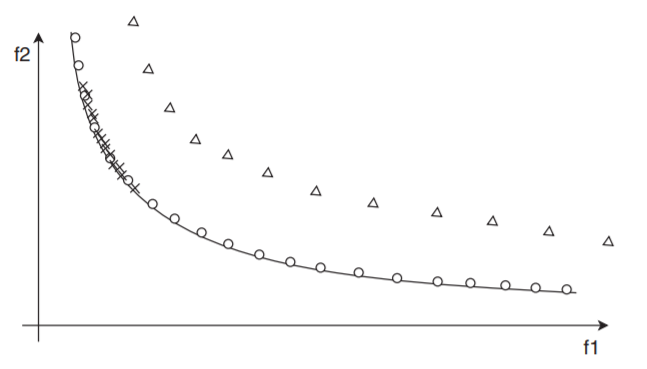
\includegraphics[width=0.75\textwidth]{assets/img/03_Konzept/Pareto.png}
    }
    \caption{Beispiel einer Pareto-Front zweier Zielfunktionen $f_1$ und $f_2$} 
    \label{img:paretofront}
    \source{\cite[vgl.][S. 286]{talbi_multi-objective_2012}}
\end{figure}

Die ausgewählten Metaheuristken entsprechen zum Zeitpunkt der Thesis den State-of-the-Art Lösungsverfahren für das \ac{mrcpsp}. Es werden die im Kapitel \ref{sec:Metaheuristiken} vorgestellten Metaheuristiken, angelehnt an den bestehenden Publikationen für das (M)\ac{rcpsp} gemäß der Problemstellung implementiert und verglichen. Des Weiteren werden die Metaheuristiken mit einem Random Solver und dem Hill Climbing-Algorithmus verglichen, welcher der naive lokale Suche entspricht:

\begin{description}
\item[Random Solver] Der Random Solver entspricht einer naiven Variante und erstellt ohne Heuristiken über das \ac{ssgs} zufällige Aktivitäts- und Modilisten. Der Random Solver dient für die Evaluation als eine Referenz, um die Ergebnisse der Metaheuriken besser vergleichen und interpretieren zu können. 

\item[Hill Climbing / \acf{LS}] Der generische \ac{LS}-Algorithmus gilt als eine weitere Referenz zwischen dem Random Solver und den Metaheuristiken. Iterativ wird über die Nachbarschaftsfunktion einer bestehenden Lösung die nächstbeste ausgewählt (vgl. Kapitel \ref{sec:Metaheuristiken}).  

\item[\acf{TS}] Die \ac{TS} wurde in unterschiedlichen Versionen bereits 1999 von \cite[S. 9]{kolisch_heuristic_1998} für das \ac{rcpsp} aufgegriffen. Eine Variante verwendet als Nachbarschaft einer Lösung eine Menge von ausgehenden Lösungen mit einzelnen Aktivitätstauschen \cite[vgl.][S. 5]{thomas_tabu_1998}. 

\item[\acf{SA}] Abermals wurde 1999 von \cite[S. 9]{kolisch_heuristic_1998} für das \ac{rcpsp} die Simulated Annealing-Metaheuristik aufgegriffen. Hierbei wurde, wie bei der \ac{TS}, die Nachbarschaft aus einzelnen Aktivitätstauschen realisiert. 

\item[\acf{GA}] Ebenfalls wurden in der Publikation von \cite[S. 9]{kolisch_heuristic_1998} für das \ac{rcpsp} eine Vielzahl an genetischen Algorithmen verglichen. Bei den Crossover Operatoren steht eine Vielzahl zur Verfügung: Darunter der One-Point Crossover, die Erweiterung, der Two-Point Crossover und die im Abschnitt \ref{subsec:Grundlagen_EvolutionäreAlgorithmen} bereits vorgestellte Uniform Crossover Operation \cite[vgl.][S. 4 f.]{hartmann_competitive_1998}. 

Als Mutation Operator können austauschbare Aktivitäten innerhalb einer Aktivitätsliste mit einer gewissen Wahrscheinlichkeit $p_{mutation}$ miteinander gewechselt werden. \cite[vgl.][S. 5]{hartmann_competitive_1998} 

Für das \ac{mrcpsp} können sowohl der Two-Point Crossover als auch der Mutation Operator genutzt werden \cite[vgl. ][S. 10 ff.]{rezaeian_using_2015}. Innerhalb dieser Thesis werden beide Operationen zur Realisierung des genetischen Algorithmus verwendet und im Abschnitt \ref{subsec:MetaheuristischeAlgorithmen_EvolutionaereAlgorithmen} erläutert.
\end{description}

Algorithmen, wie die \ac{LS}, \ac{TS} und \ac{SA} sehen alle eine Nachbarschaftsfunktion $N(s)$ vor. Diese wird innerhalb der Arbeit für alle Verfahren gleichermaßen implementiert. Aufgrund der möglichen hohen Anzahl an Kombinationen innerhalb einer Nachbarschaft, soll nur eine Teilmenge $\tilde{N}(s) \subset N(s)$ betrachtet werden. Dies geht aus der Publikation von \cite[S. 5]{thomas_tabu_1998} hervor. \\

Eine Publikation für das Lösen des \ac{mrcpsp} mithilfe von Simulated Annealing beschreibt drei Möglichkeiten zur Bildung einer Nachbarschaftsfunktion. Aktivitäten können innerhalb der Aktivitätsliste samt deren Modi verschoben werden. Zudem existiert die Möglichkeit, dass eine Aktivität zufällig selektiert wird und der zugehörige Modus auf einen anderen Modus geändert werden kann. Die dritte Variante stellt die Kombination der beiden vorherigen Varianten dar, welche in dieser Arbeit als Nachbarschaftsfunktion aufgegriffen wird. \cite[vgl.][S. 145]{jozefowska_simulated_2001}